\documentclass{article}
\usepackage[italian]{babel}
\usepackage{graphicx}
\usepackage{amsmath}
\usepackage{booktabs}

\title{Gradiente Elettrochimico, Diffusione e Trasporti}
\author{Orcam}
\date{}

\begin{document}

\maketitle

\section{Diffusione}
La diffusione è il processo di dispersione di molecole da zone a concentrazione più alta a zone a concentrazione più bassa, guidato dal movimento termico casuale. Nonostante sia un processo lento, nelle cellule avviene in frazioni di millisecondo.

\subsection{Equazione di Fick}
Il flusso di diffusione è descritto dall'equazione di Fick:
\[
dQ_s = D_s \times A \times dC_s
\]
dove:
\begin{itemize}
    \item \(dQ_s\) è la quantità di sostanza che diffonde,
    \item \(D_s\) è il coefficiente di diffusione,
    \item \(A\) è l'area della membrana,
    \item \(dC_s\) è la differenza di concentrazione.
\end{itemize}

\begin{figure}[h]
    \centering
    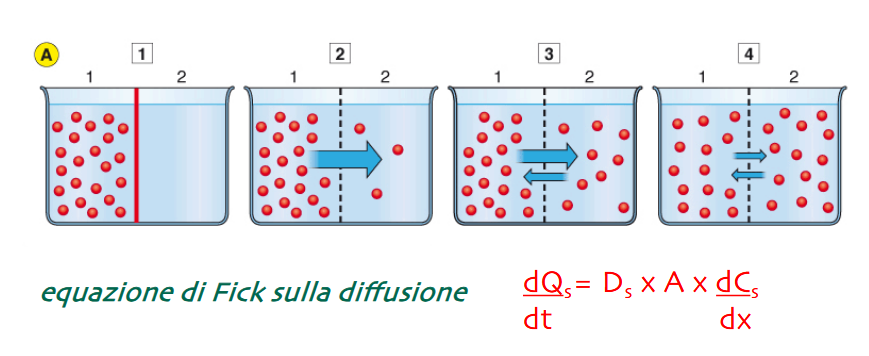
\includegraphics[width=1\textwidth]{Neuroscienze 2024-2025/Modulo I/Immagini Modulo I/Screenshot 2025-06-21 at 16-22-28 4. Gradiente elettrochimico_Diffusione facilitata_trasporti.pdf.png}
    \caption{Illustrazione del processo di diffusione attraverso una membrana.}
    \label{fig:diffusione}
\end{figure}

\section{Flusso di Membrana}
Il flusso di membrana \(J\) è definito come:
\[
J = \frac{dQ_s}{dt} \quad (\text{mol/cm}^2/\text{sec})
\]
La permeabilità della membrana \(P\) è data da:
\[
P = \frac{D_m K_s}{x}
\]
dove:
\begin{itemize}
    \item \(D_m\) è il coefficiente di diffusione nella membrana,
    \item \(K_s\) è il coefficiente di ripartizione,
    \item \(x\) è lo spessore della membrana.
\end{itemize}

\section{Permeabilità della Membrana}
La membrana plasmatica è una barriera selettiva. Le sue caratteristiche di permeabilità includono:
\begin{itemize}
    \item Gas (es. \(O_2\), \(CO_2\)),
    \item Molecole idrofobiche (es. benzene),
    \item Piccole molecole polari (es. \(H_2O\)),
    \item Grosse molecole polari e ioni (es. glucosio, \(Na^+\), \(K^+\)).
\end{itemize}

\section{Trasporti Passivi e Attivi}
\subsection{Trasporto Passivo}
\begin{itemize}
    \item \textbf{Diffusione semplice}: avviene secondo gradiente di concentrazione.
    \item \textbf{Diffusione facilitata}: mediata da proteine di membrana (trasportatori o canali ionici).
\end{itemize}

\subsection{Trasporto Attivo}
\begin{itemize}
    \item Avviene contro gradiente di concentrazione o elettrico.
    \item Richiede energia (ATP).
    \item Esempio: pompa \(Na^+/K^+\)-ATPasi.
\end{itemize}

\begin{figure}[h]
    \centering
    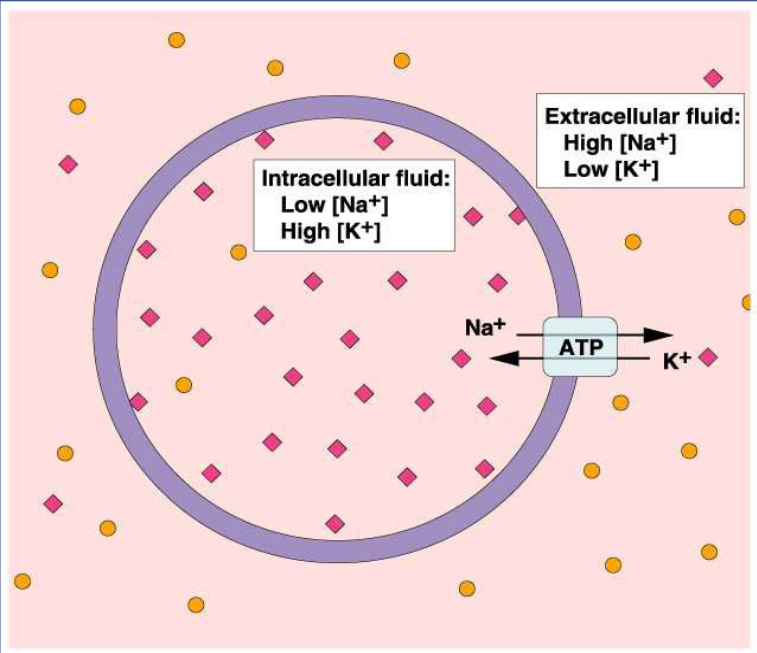
\includegraphics[width=1\textwidth]{Neuroscienze 2024-2025/Modulo I/Immagini Modulo I/Screenshot 2025-06-21 at 16-23-00 4. Gradiente elettrochimico_Diffusione facilitata_trasporti.pdf.png}
    \caption{Meccanismo della pompa \(Na^+/K^+\)-ATPasi.}
    \label{fig:pompa}
\end{figure}

\section{Diffusione Facilitata}
\subsection{Trasportatori}
I trasportatori mediano il passaggio di molecole specifiche attraverso la membrana. Possono essere:
\begin{itemize}
    \item \textbf{Uniporto}: trasporto di una sola sostanza in una direzione.
    \item \textbf{Simporto}: trasporto di due sostanze nella stessa direzione.
    \item \textbf{Antiporto}: trasporto di due sostanze in direzioni opposte.
\end{itemize}

\subsection{Canali Ionici}
\begin{itemize}
    \item Consentono il passaggio di ioni secondo gradiente elettrochimico.
    \item Sono altamente selettivi per carica e dimensione.
    \item Possono essere passivi o regolati da stimoli (es. voltaggio, ligandi).
\end{itemize}

\begin{figure}[h]
    \centering
    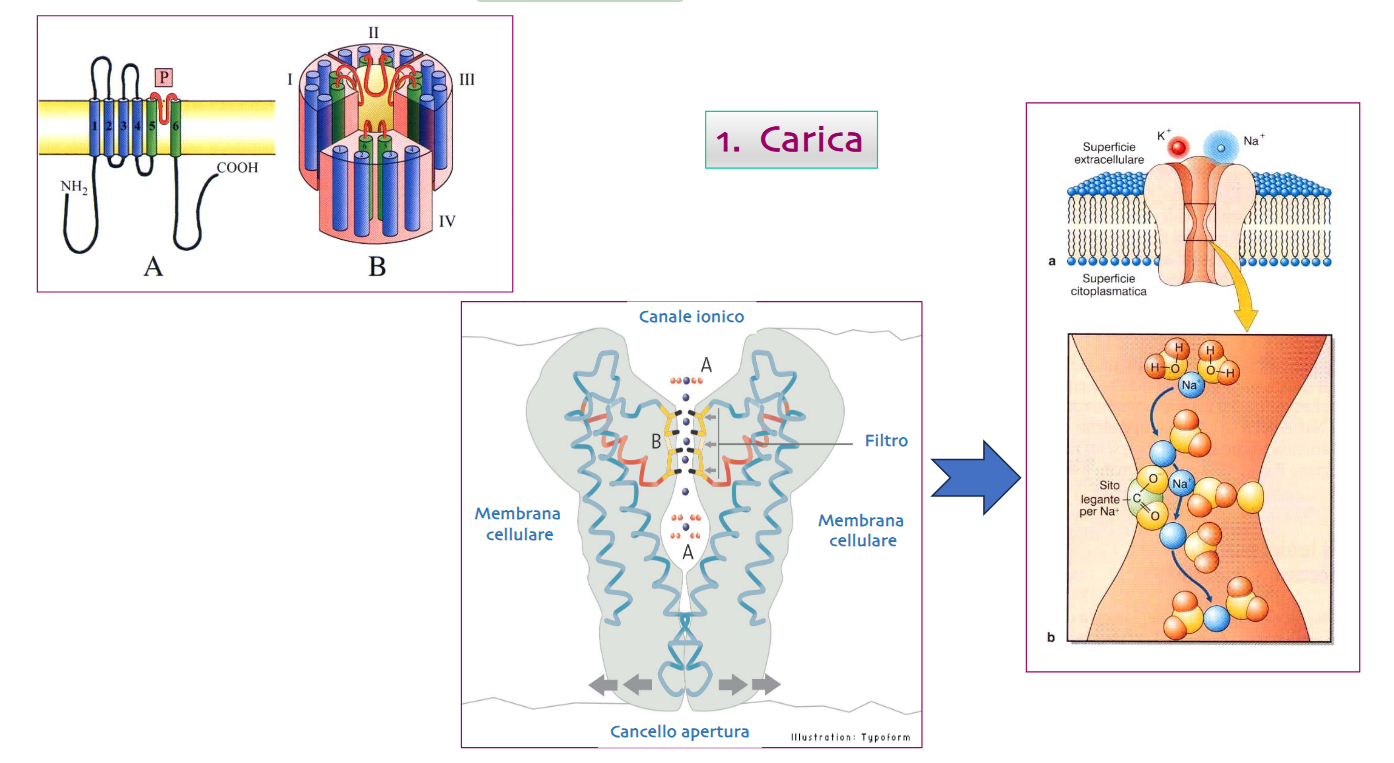
\includegraphics[width=1\textwidth]{Neuroscienze 2024-2025/Modulo I/Immagini Modulo I/Screenshot 2025-06-21 at 17-11-44 4. Gradiente elettrochimico_Diffusione facilitata_trasporti.pdf.png}
    \caption{Struttura e funzionamento dei canali ionici.}
    \label{fig:canali}
\end{figure}

\section{Trasporti Attivi Primari}
\subsection{Pompa \(Na^+/K^+\)-ATPasi}
\begin{itemize}
    \item Mantiene i gradienti di \(Na^+\) e \(K^+\) tra intra- ed extra-cellula.
    \item Trasporta 3 \(Na^+\) fuori e 2 \(K^+\) dentro per ogni ATP idrolizzato.
    \item Fondamentale per l'eccitabilità neuronale.
\end{itemize}

\section{Endocitosi ed Esocitosi}
\subsection{Esocitosi}
\begin{itemize}
    \item Secrezione di proteine e lipidi mediante vescicole.
    \item Può essere costitutiva o regolata da segnali esterni.
\end{itemize}

\subsection{Endocitosi}
\begin{itemize}
    \item Internalizzazione di molecole mediante vescicole rivestite di clatrina.
    \item Mediata da recettori specifici.
\end{itemize}

\begin{figure}[h]
    \centering
    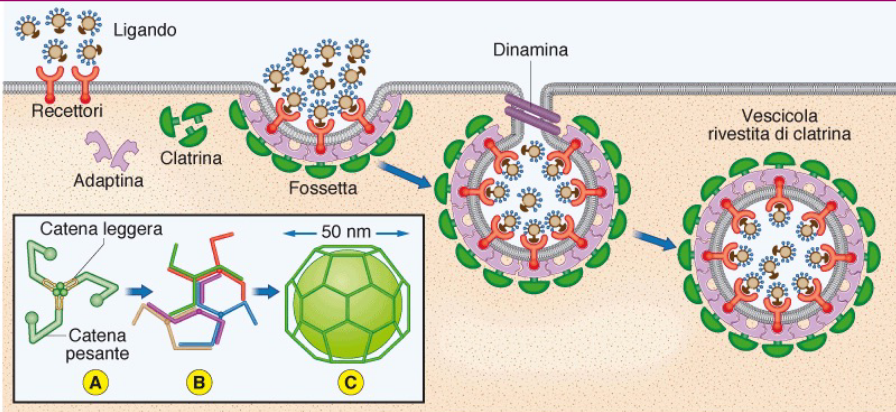
\includegraphics[width=1\textwidth]{Neuroscienze 2024-2025/Modulo I/Immagini Modulo I/Screenshot 2025-06-21 at 17-13-17 4. Gradiente elettrochimico_Diffusione facilitata_trasporti.pdf.png}
    \caption{Processo di endocitosi mediata da recettore.}
    \label{fig:endocitosi}
\end{figure}

\end{document}